\documentclass{article}
\usepackage{josuamathheader}
\newcommand{\rot}{\operatorname{rot}}
\renewcommand{\div}{\operatorname{div}}
\begin{document}
\section*{Aufgabe 2}
\begin{enumerate}[(a)]
    \item Für das Linienintegral erhalten wir durch Parametrisierung $r = r(\varphi) = \begin{pmatrix}
        \cos(\varphi)\\\sin(\varphi)\\0
    \end{pmatrix}$ folgendes Ergebnis
    \begin{align*}
        \oint_\mathcal{C} v(r) \intd r &= \int_0^{2\pi} v(r(\varphi))\cdot r'(\varphi) \intd \varphi
        \intertext{Unter Ausnutzung von $\cos^2 + \sin^2 = 1$ in $v(r(\varphi))$ erhalten wir folgenden Ausdruck}
        &= \int_0^{2\pi} \begin{pmatrix}
            -\sin(\varphi)\\
            \cos(\varphi)\\
            0
        \end{pmatrix} \cdot \begin{pmatrix}
            -\sin(\varphi)\\
            \cos(\varphi)\\
            0
        \end{pmatrix} \intd \varphi\\
        &= \int_0^{2\pi} 1 \intd \varphi\\
        &= 2\pi
    \end{align*}
    Daraufhin berechnen wir die Rotation von $v$.
    \begin{align*}
        \rot v(r) &= \nabla \times v(r)\\
        &= \begin{pmatrix}
            \partial_y(xz) - \partial_z (x^2 + y^2x)\\
            \partial_z(-(x^2 + y^2)y) - \partial_y(xz)\\
            \partial_x((x^2 + y^2)x) + \partial_y((x^2 + y^2)y)
        \end{pmatrix}\\
        &= \begin{pmatrix}
            0\\
            0\\
            3x^2 + y^2 + 3y^2 + x^2
        \end{pmatrix}\\
        &= \begin{pmatrix}
            0\\0\\4(x^2+y^2)
        \end{pmatrix}\\
        &= \begin{pmatrix}
            0\\0\\4r^2
        \end{pmatrix}.
    \end{align*}
    Nun berechnen wir das Integral über $\mathcal{F}$.
    \begin{align*}
        \int_\mathcal{F} \intd A \rot v(r) &= \int_0^1 \int_0^{2\pi} \begin{pmatrix}
            0\\0\\1
        \end{pmatrix} \cdot \begin{pmatrix}
            0\\
            0\\
            4r^2
        \end{pmatrix} \cdot r \intd \varphi \intd r\\
        &= 2\pi \int_0^1 4r^2 \cdot r \intd r\\
        &= 2\pi r^4 \bigg|_0^1\\
        &= 2\pi
    \end{align*}
    Dies bestätigt den Satz von Stokes.
    \item Wir berechnen zunächst den Fluss von $v$ durch die einzelnen Oberflächen des Würfels. Das sind insgesamt 6 Integrale.
    \begin{enumerate}[(i)]
        \item $\oint_{\partial V, x = 0} \begin{pmatrix}
            -(x^2 + y^2)y\\
            (x^2 + y^2)x\\
            xz
        \end{pmatrix} \intd \vec A = \int_0^1 \int_0^1 \begin{pmatrix}
            -(y^2)y\\
            0\\
            0
        \end{pmatrix} \cdot \begin{pmatrix}
            -1\\0\\0
        \end{pmatrix} \intd y \intd z = \int_0^1 y^3 \intd y =\frac{1}{4}$.
        \item $\oint_{\partial V, x = 1} \begin{pmatrix}
            -(x^2 + y^2)y\\
            (x^2 + y^2)x\\
            xz
        \end{pmatrix} \intd \vec A = \int_0^1 \int_0^1 \begin{pmatrix}
            -(1 + y^2)y\\
            1 + y^2\\
            z
        \end{pmatrix} \cdot \begin{pmatrix}
            1\\0\\0
        \end{pmatrix} \intd y \intd z = \int_0^1 -y - y^3 \intd y = -\frac{3}{4}$.
        \item $\oint_{\partial V, y = 0} \begin{pmatrix}
            -(x^2 + y^2)y\\
            (x^2 + y^2)x\\
            xz
        \end{pmatrix} \intd \vec A = \int_0^1 \int_0^1 \begin{pmatrix}
            0\\
            x^3\\
            xz
        \end{pmatrix} \cdot \begin{pmatrix}
            0\\-1\\0
        \end{pmatrix} \intd x \intd z = \int_0^1 -x^3 \intd x =-\frac{1}{4}$.
        \item $\oint_{\partial V, y = 1} \begin{pmatrix}
            -(x^2 + y^2)y\\
            (x^2 + y^2)x\\
            xz
        \end{pmatrix} \intd \vec A = \int_0^1 \int_0^1 \begin{pmatrix}
            -(x^2 + 1)\\
            x^3 + x\\
            xz
        \end{pmatrix} \cdot \begin{pmatrix}
            0\\1\\0
        \end{pmatrix} \intd x \intd z = \int_0^1 x^3 + x \intd x =\frac{3}{4}$.
        \item $\oint_{\partial V, z = 0} \begin{pmatrix}
            -(x^2 + y^2)y\\
            (x^2 + y^2)x\\
            xz
        \end{pmatrix} \intd \vec A = \int_0^1 \int_0^1 \begin{pmatrix}
            -(x^2 + y^2)y\\
            (x^2 + y^2)x\\
            0
        \end{pmatrix} \cdot \begin{pmatrix}
            0\\0\\-1
        \end{pmatrix} \intd x \intd z = \int_0^1 0 \intd x =0$.
        \item $\oint_{\partial V, z = 1} \begin{pmatrix}
            -(x^2 + y^2)y\\
            (x^2 + y^2)x\\
            xz
        \end{pmatrix} \intd \vec A = \int_0^1 \int_0^1 \begin{pmatrix}
            -(x^2 + y^2)y\\
            (x^2 + y^2)x\\
            x
        \end{pmatrix} \cdot \begin{pmatrix}
            0\\0\\1
        \end{pmatrix} \intd x \intd z = \int_0^1 x \intd x =\frac{1}{2}$.
    \end{enumerate}
    Die Summe dieser 6 Integrale ist $\frac{1}{2}$. Nun berechnen wir die Divergenz von $v$.
    \[
        \div v(r) = -2xy + 2xy + x = x.  
    \]
    Das Integral über die Divergenz ist also
    \[
        \int_{\partial V} \intd V x = \int_0^1 \int_0^1 \int_0^1 x \intd x \intd y \intd z = \int_0^1 \int_0^1 \frac{1}{2} \intd y\intd z = \frac{1}{2}. 
    \]
    Damit ist auch in diesem Beispiel der Gauss'sche Satz wahr.
    \item Siehe Abbildung 1, 2 und 3.
\end{enumerate}
\begin{figure}
    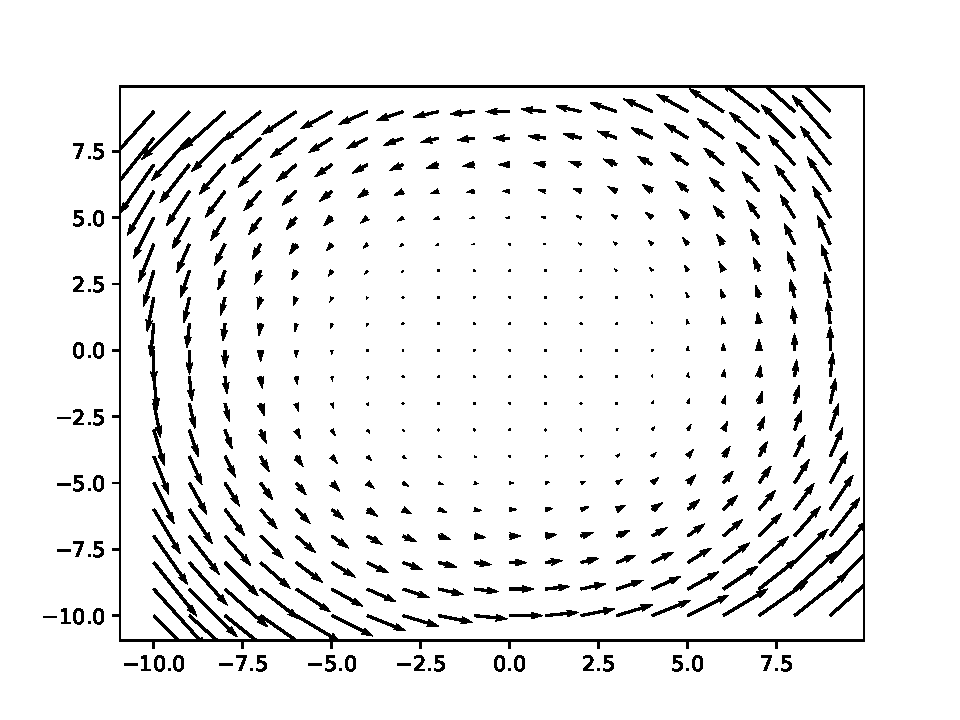
\includegraphics{xy-Ebene.pdf}
    \caption{xy-Ebene}
\end{figure}
\begin{figure}
    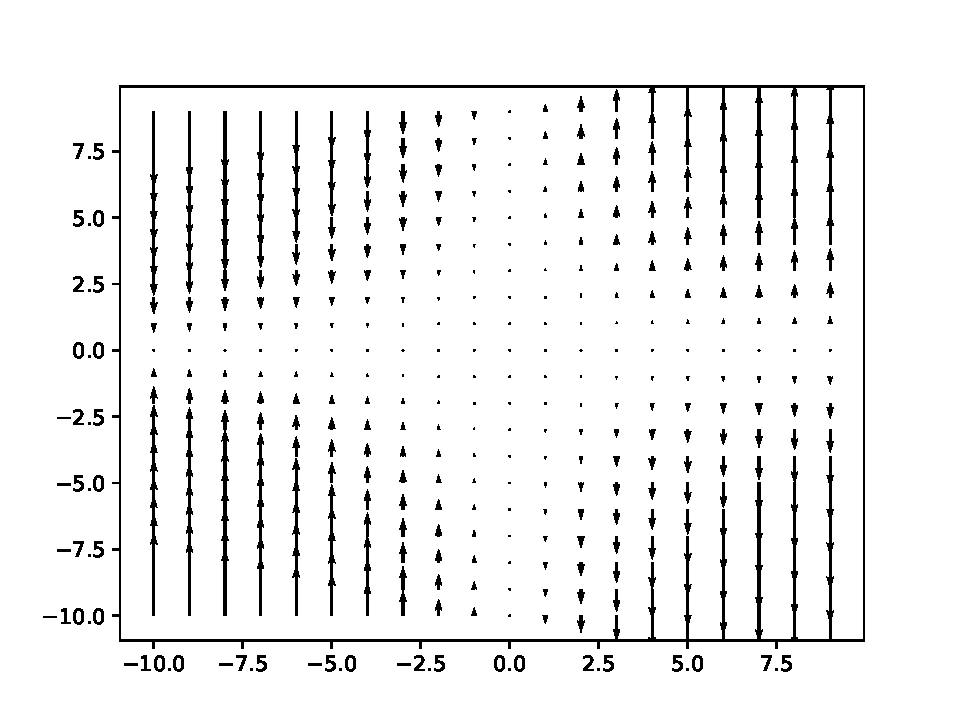
\includegraphics{xz-Ebene.pdf}
    \caption{xz-Ebene}
\end{figure}
\begin{figure}
    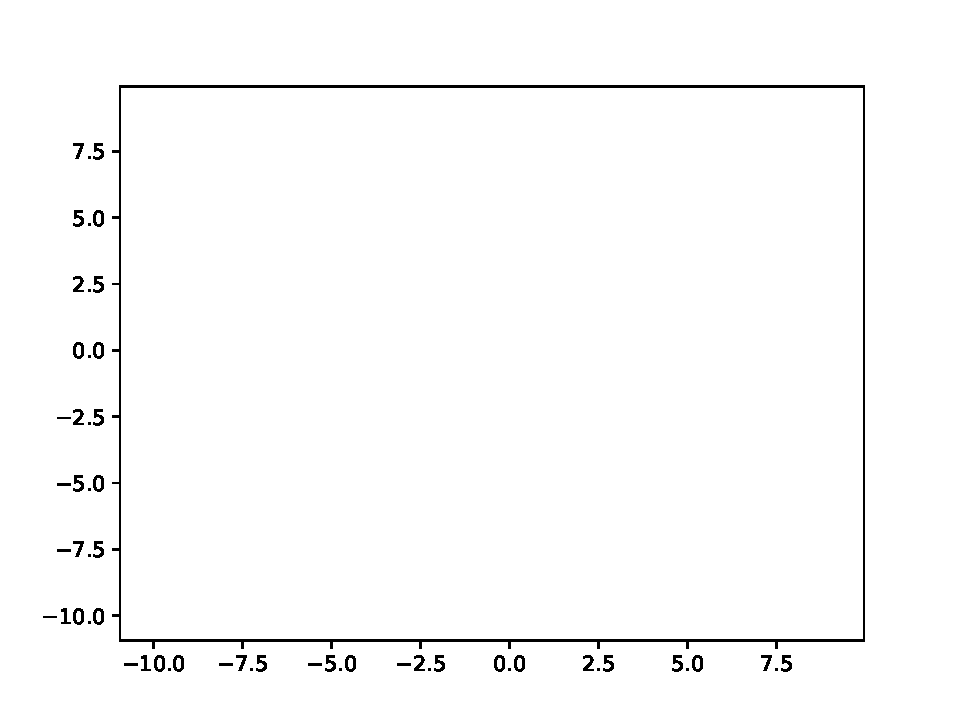
\includegraphics{yz-Ebene.pdf}
    \caption{yz-Ebene}
\end{figure}
\end{document}